%-------------------------------------------------------------------------------
%                             ADDITIONAL PACKAGES
%-------------------------------------------------------------------------------
\documentclass[
  letterpaper, 
%   showframes,
%   vline=2.2em,
  maincolor=black,
  sectioncolor=black!90,
  subsectioncolor=black!70,
  itemtextcolor=black!40,
%   sidebarwidth=0.4\paperwidth,
%   topbottommargin=0.03\paperheight,
%   leftrightmargin=20pt,
%   proilepicsize=4.5cm,
]{fortysecondscv}


\usepackage[T1]{fontenc}
\usepackage[utf8]{inputenc}


\usepackage[spanish]{babel}
\usepackage{graphicx}
\usepackage{fancyhdr}
\usepackage{blindtext}
\usepackage{geometry}
\usepackage{array}
\usepackage{multicol}
\usepackage{vwcol} 
\usepackage{tabulary}
\usepackage{url}
\usepackage{float}

% improve word spacing and hyphenation
\usepackage{microtype}
\usepackage{ragged2e}

% take care of proper font encoding
\ifxetexorluatex
	\usepackage{fontspec}
	\defaultfontfeatures{Ligatures=TeX}
% \newfontfamily\headingfont[Path = fonts/]{segoeuib.ttf} % local font
\else
	\usepackage[utf8]{inputenc}
	\usepackage[T1]{fontenc}
% \usepackage[sfdefault]{noto} % use noto google font
\fi

% enable mathematical syntax for some symbols like \varnothing
\usepackage{amssymb}

% bubble diagram configuration
\usepackage{smartdiagram}
\smartdiagramset{
  % defaut font size is \large, so adjust to harmonize with sidebar layout
  bubble center node font = \footnotesize,
  bubble node font = \footnotesize,
  % default: 4cm/2.5cm; make minimum diameter relative to sidebar size
  bubble center node size = 0.4\sidebartextwidth,
  bubble node size = 0.25\sidebartextwidth,
  distance center/other bubbles = 1.5em,
  % set center bubble color
  bubble center node color = maincolor!70,
  % define the list of colors usable in the diagram
  set color list = {maincolor!10, maincolor!40,
  maincolor!20, maincolor!60, maincolor!35},
  % sets the opacity at which the bubbles are shown
  bubble fill opacity = 0.8,
}


%-------------------------------------------------------------------------------
%                            PERSONAL INFORMATION
%-------------------------------------------------------------------------------
%%
%
% \cvprofilepic{img/logoUCR.png}

\cvname{\begin{center}
\includegraphics[width=0.5\textwidth]{img/logoUCR.png}
\\\vspace{-0mm}Universidad de\\Costa Rica\end{center}}

\cvjobtitle{\begin{center}
\includegraphics[width=0.5\textwidth]{img/logoEIE.png}\\\vspace{-0mm}Escuela de\\Ingeniería Eléctrica\end{center}}

%% optional information


% NOTE: ordering in sidebar will mimic the following order
% date of birth
% \cvbirthday{\textit{M. Sc.} Ricardo Román-Brenes}
% short address/location, use \newline if more than 1 line is required
% \cvaddress{\url{ricardo.roman@ucr.ac.cr}}
% phone number


%-------------------------------------------------------------------------------
%                              SIDEBAR 1st PAGE
%-------------------------------------------------------------------------------
% add more profile sections to sidebar on first page
\addtofrontsidebar{
	% include gosquare national flags from https://github.com/gosquared/flags;
	% naming according to ISO 3166-1 alpha-2 country codes

	% social network accounts incl. proper hyperlinks
	\profilesection{Estudiantes}
		\begin{icontable}{2em}{1em}
		    % overleaf still not supports Academicons and FontAwesome5 for XeLaTeX, which contain the overleaf logl...unbelievable...
		    %\social{\aiOverleafSquare}
			\social{\faUser}
				{}
				{\textit{} Gabriel Araya Mora}
			\social{\faAt}
				{}
				{\url{gabomora2200@gmail.com}}
			\social{\faUser}
			    {}
			    {\textit{} Ignacio Montenegro}
		    \social{\faAt}
				{}
				{\url{imonte00@gmail.com}}
			\social{\faUser}
			    {}
			    {\textit{} Andrés Arias Campos}
		    \social{\faAt}
				{}
				{\url{andres.ariascampos@ucr.ac.cr}}
			
		\end{icontable}
		

	 
       
    
}

\addtobacksidebar{
	% include gosquare national flags from https://github.com/gosquared/flags;
	% naming according to ISO 3166-1 alpha-2 country codes

	% social network accounts incl. proper hyperlinks
	\profilesection{Docente}
		\begin{icontable}{2.5em}{1em}
		    % overleaf still not supports Academicons and FontAwesome5 for XeLaTeX, which contain the overleaf logl...unbelievable...
		    %\social{\aiOverleafSquare}
			\social{\faUser}
				{}
				{\textit{M. Sc.} Ricardo Román-Brenes}
			\social{\faAt}
				{}
				{\url{ricardo.roman@ucr.ac.cr}}
		\end{icontable}
		
}


%-------------------------------------------------------------------------------
%                         TABLE ENTRIES RIGHT COLUMN
%-------------------------------------------------------------------------------
\begin{document}

\makefrontsidebar


\cvsection{\huge \texttt{IE-0117} \textbf{Programacion bajo plataformas abiertas}}
\cvsubsection{\huge Laboratorio 4: Programando en C}
% \begin{cvtable}[1.5]
% 	\cvitem{2009 -- 2010}{Post-Doc Panda Studies}{Panda Academy}
% 		{In-depth studies on the impact of bamboo nutrition for young pandas and
% 		its relation to relaxing, sleeping and snoozing parts of the day.}
% 	\cvitem{2008 -- 2009}{Research Stay Europe}{European Panda Labs}
% 		{Spending one year abroad teaching european panda facilities about the
% 		newest findings and research in the field of asian rice hat covers and
% 		applications for bamboo as a material.}
% \end{cvtable}

% \cvsignature
    \section{Valor absoluto de un número}
    En este punto se creó una función con un if para obtener el valor absoluto de cualquier número, ya sea de tipo entero o flotante. En este caso se usó de prueba el número -48234 y como se observa en la figura 2 efectivamente calcula su valor absoluto.  
    
    
            \begin{figure}[H]
                \centering
                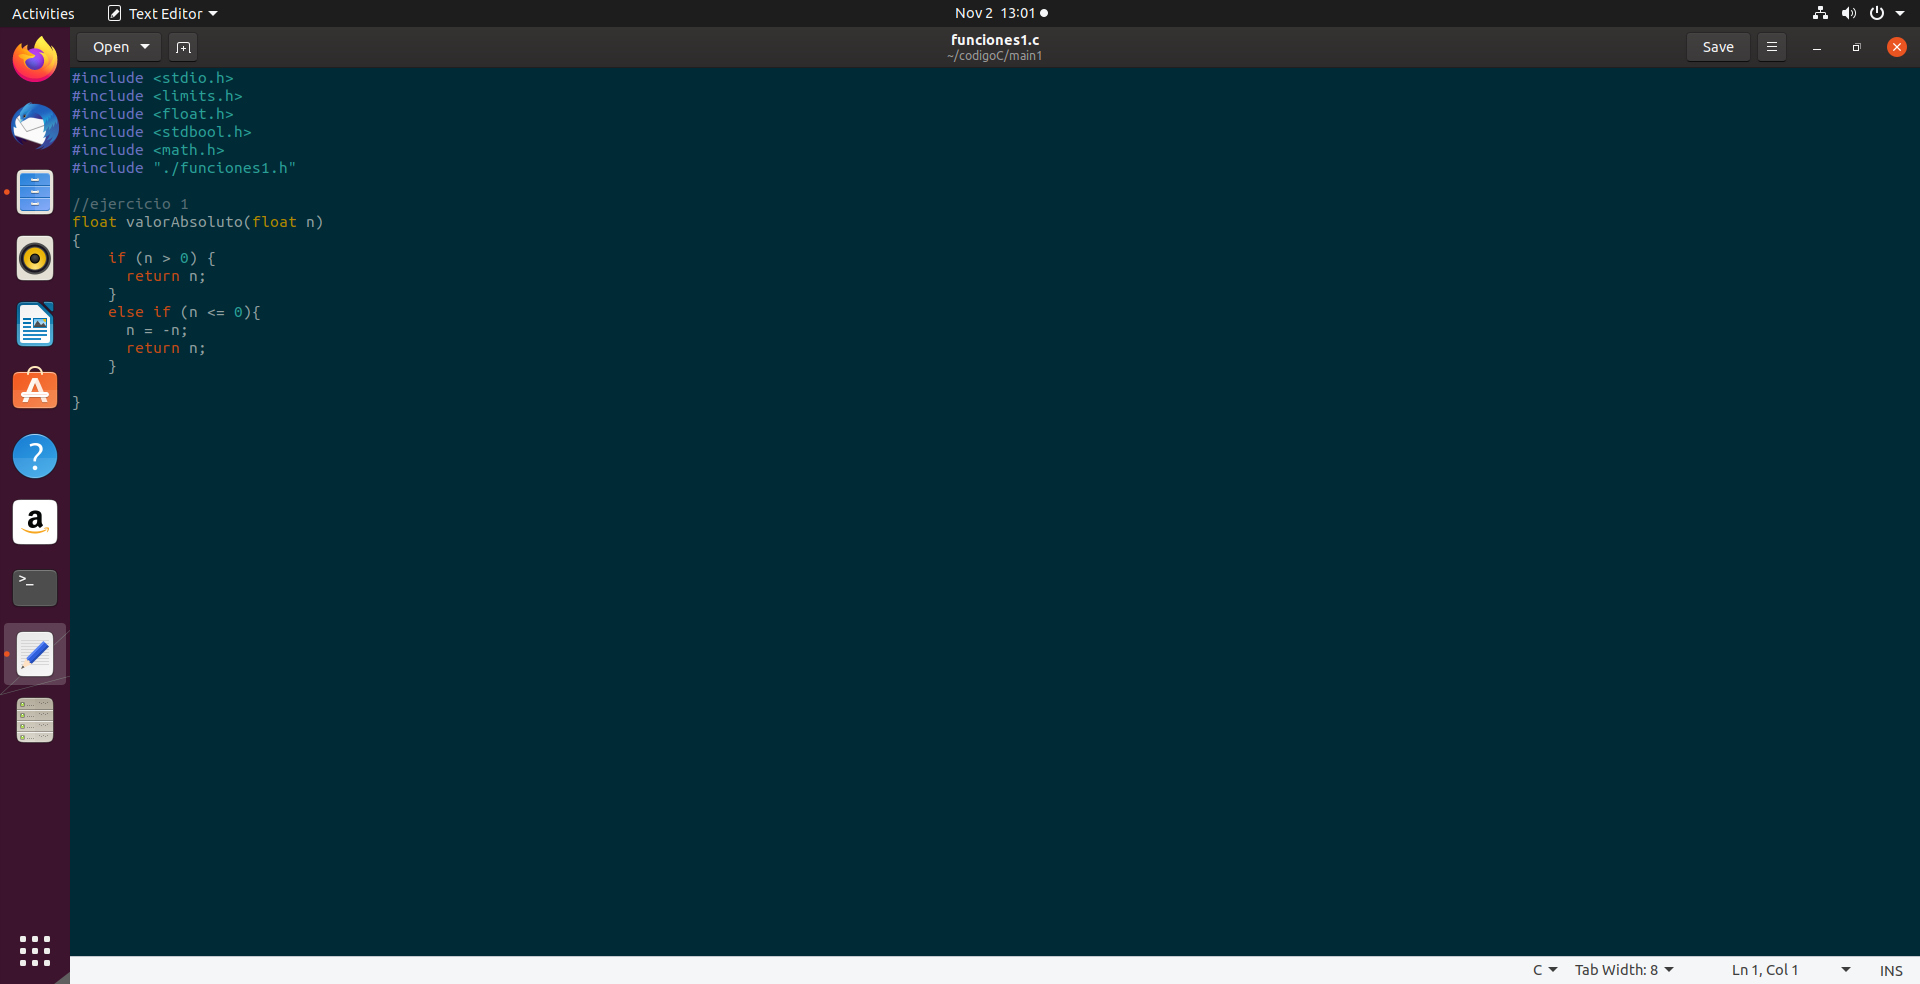
\includegraphics[trim= 0 550 1100 0,clip,width=1.20\textwidth]{img/punto1.png}
                \caption{Código para obtener el valor absoluto de un número dado }
                \label{fig:my_label}
            \end{figure}
            \begin{figure}[H]
                \centering
                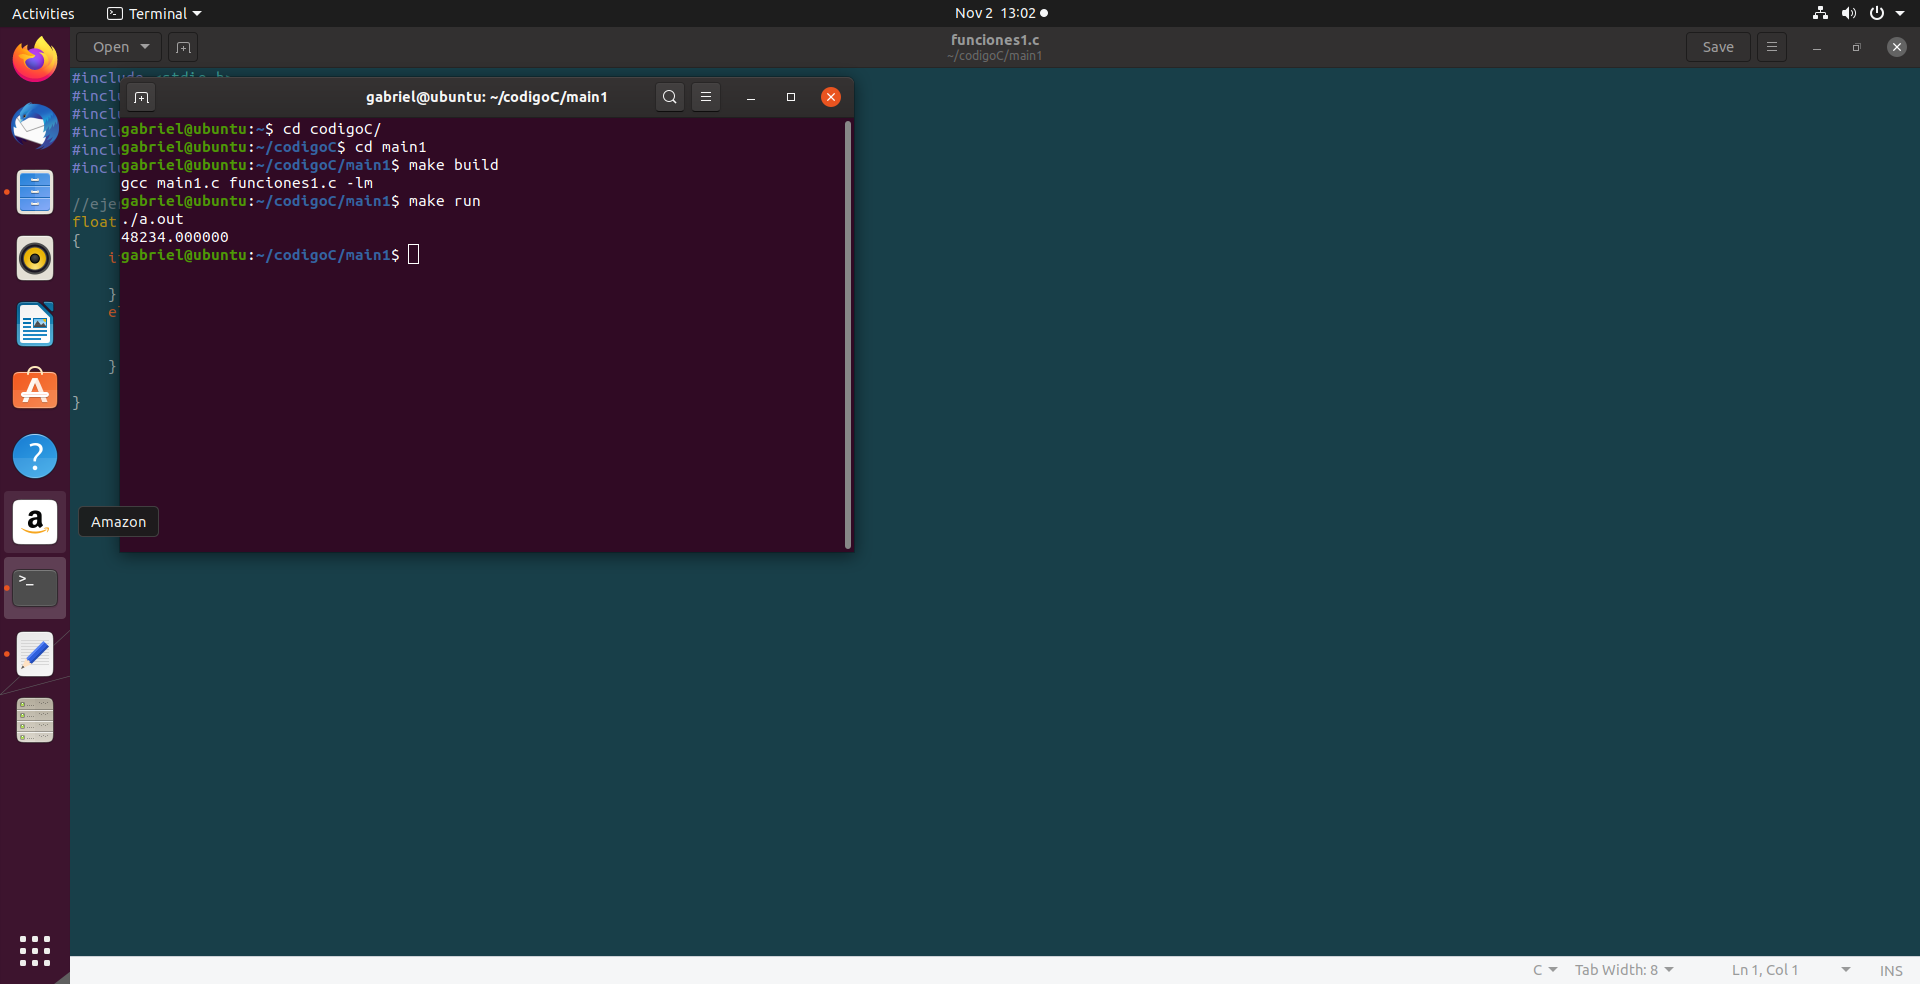
\includegraphics[trim= 115 550 950 100,clip,width=1.20\textwidth]{img/punto1-1.png}
                \caption{Valor absoluto de un número dado}                
                \label{fig:my_label}
            \end{figure}
    \newpage
        
    \section{Promoción de entradas de un videoclub}
        Se invoca la función y como parámetros se coloca el precio de las entradas. Los parámetros son de tipo float, esto para que se pueda introducir el precio que el usuario guste sin restrcciones extras. Mediante una serie de "if" y "else if" se logro que el programa reconozca solo los dos precios más bajos.
        
            \begin{figure}[H]
                \centering
                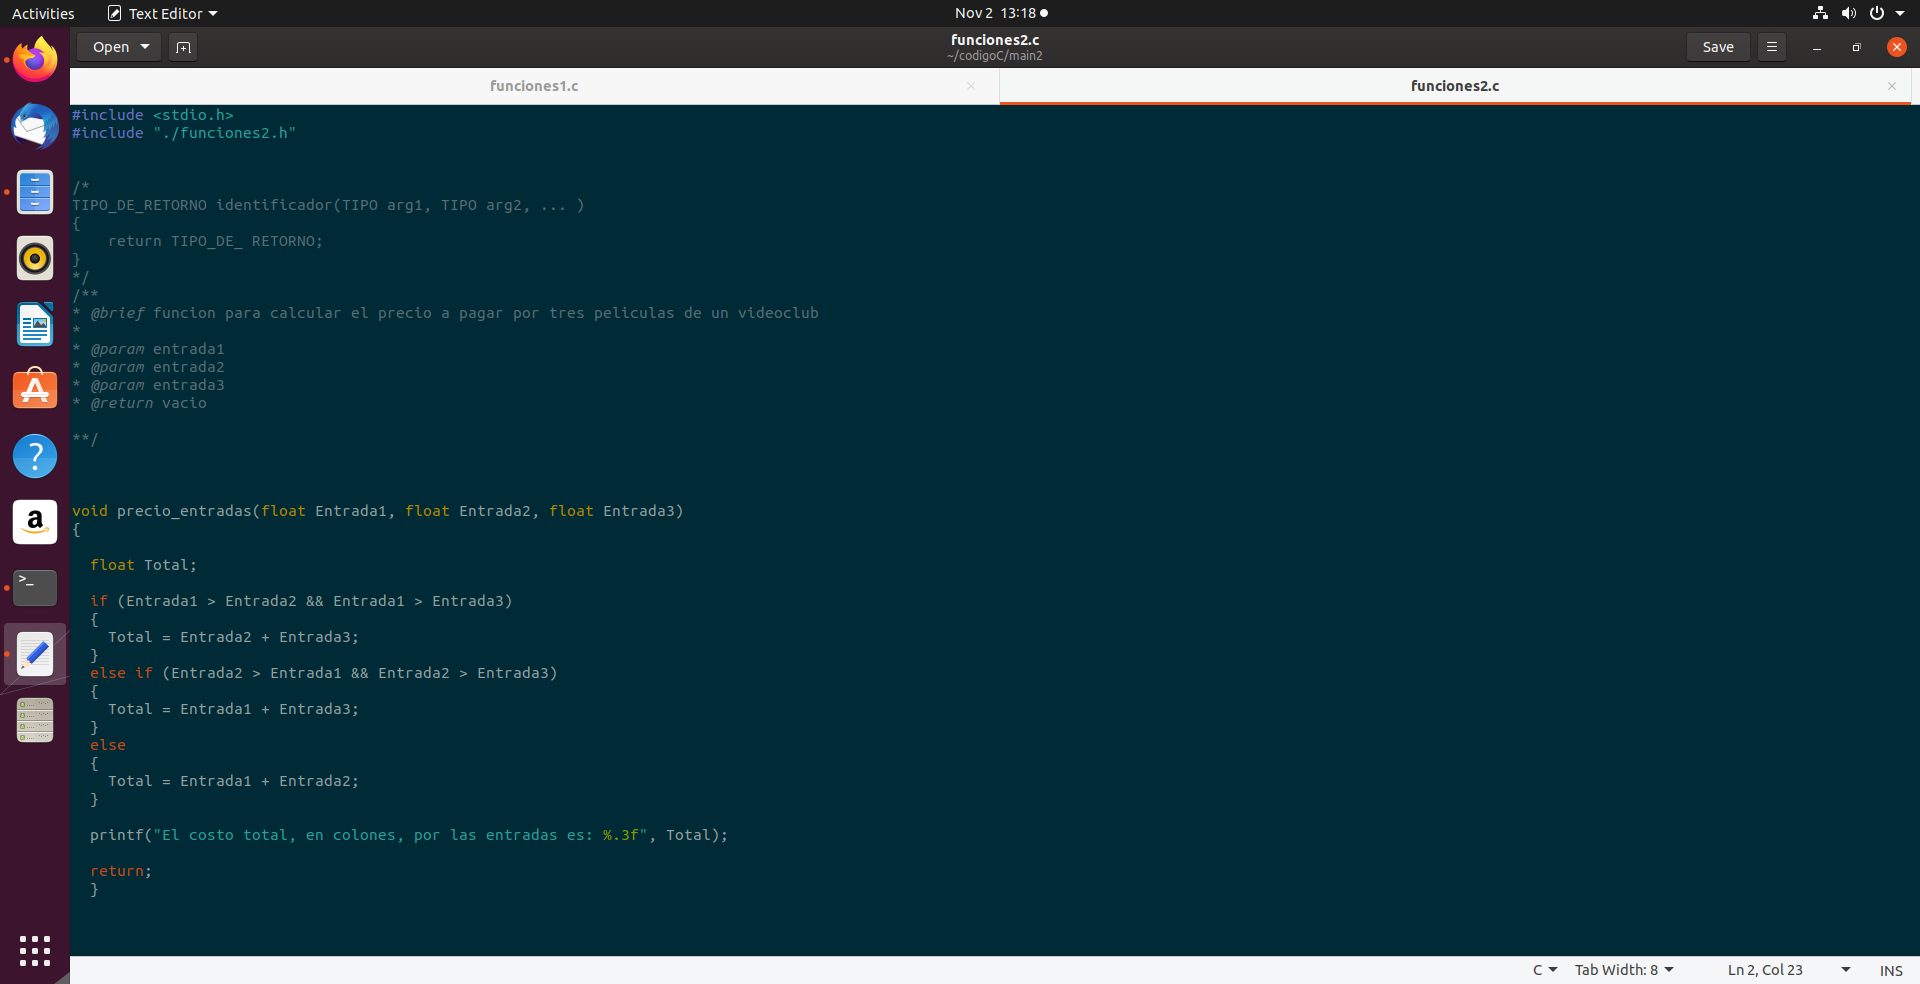
\includegraphics[trim= 50 50 850 100,clip,width=1.20\textwidth]{img/punto2.png}
                \caption{Promocion de entradas de un videoclub}
                \label{fig:my_label}
            \end{figure}
            \begin{figure}[H]
                \centering
                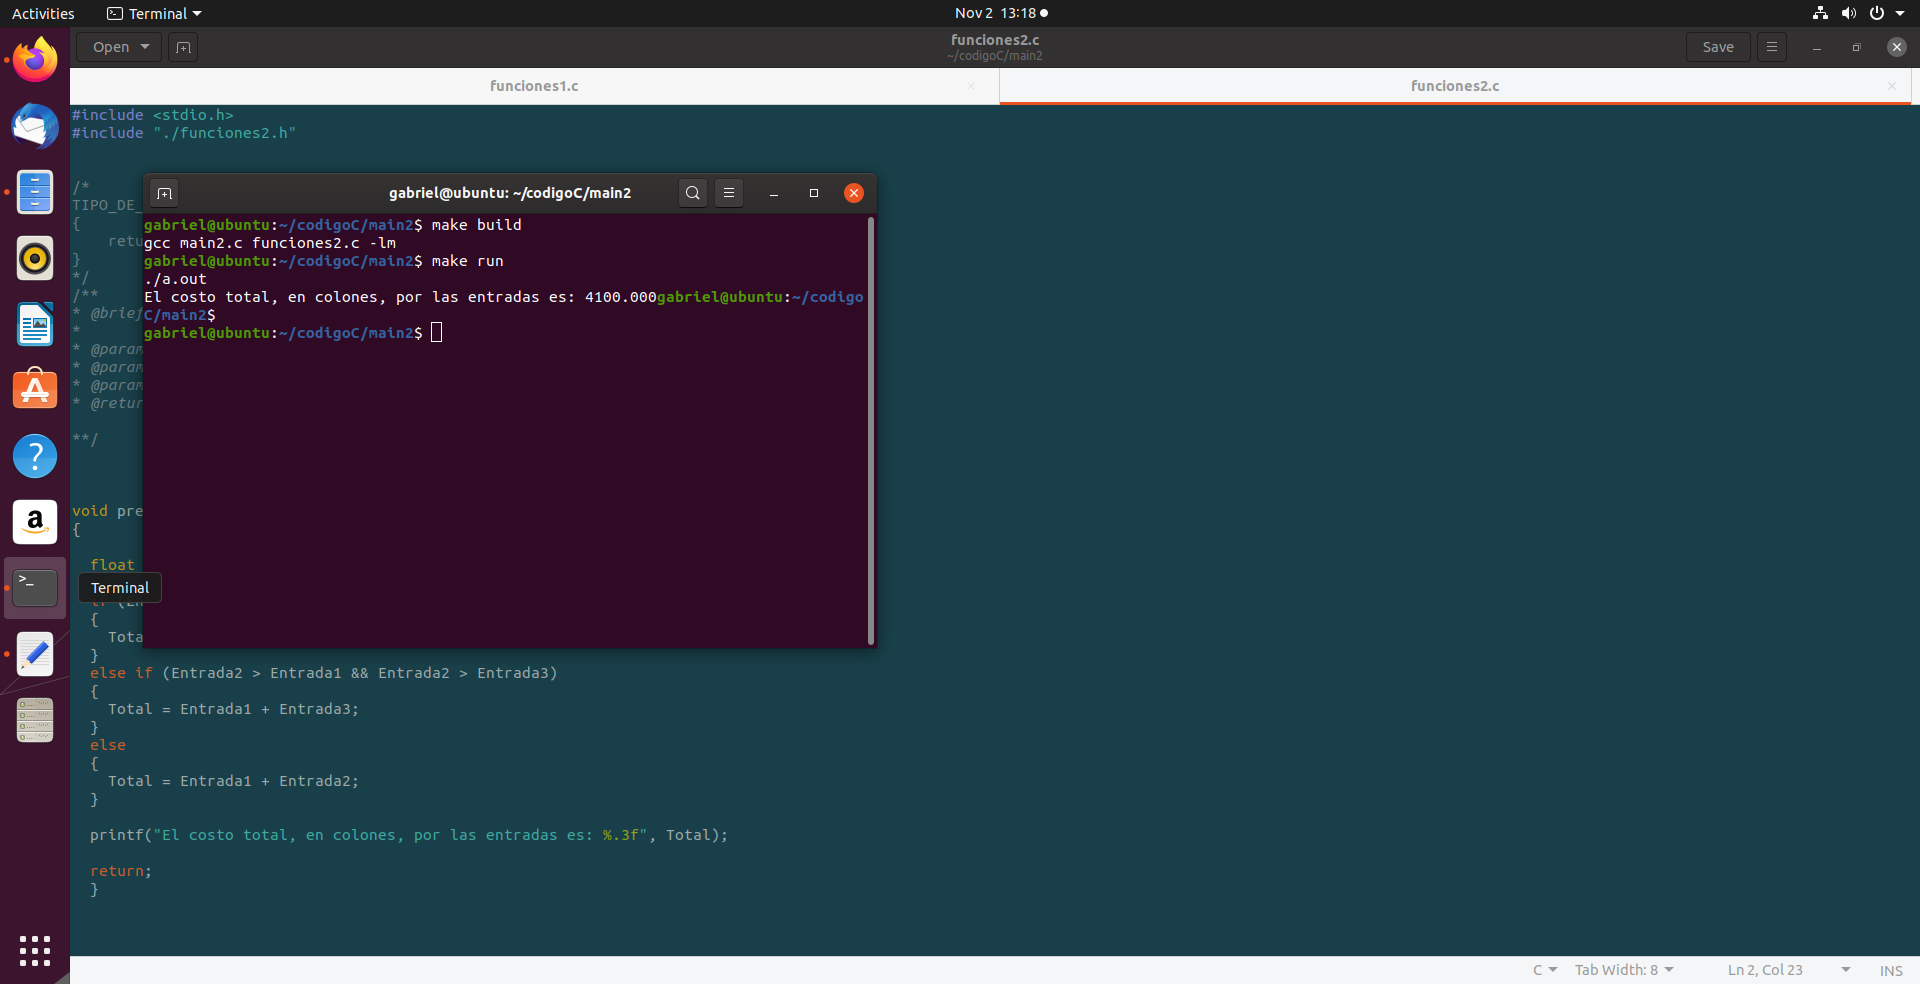
\includegraphics[trim= 140 500 900 150,clip,width=1.20\textwidth]{img/punto2-2.png}
                \caption{Salida del programa para el ejercicio 2}
                \label{fig:my_label}
            \end{figure}
            
    \section{Administrador de notas para un alumno}
        Para este ejercicio se usó el tipo de datos int <<entero>> para las notas, ya que se asumió que solo asi podrían ser estas entradas. para el promedio se usó el float <<flotante>> ya que el tiene parte fraccionaria.
        
        \begin{figure}[H]
            \centering
            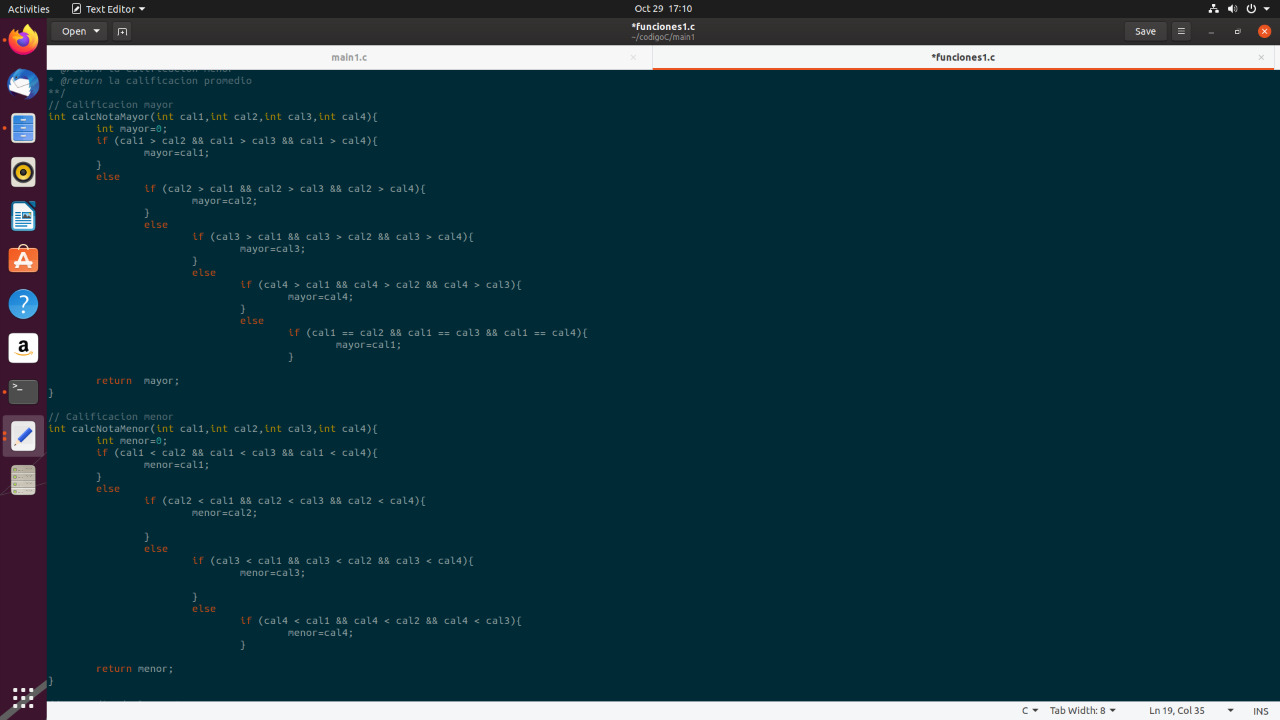
\includegraphics[trim= 0 30 580 0,clip,width=1.20\textwidth]{img/punto3.jpg}
            \caption{Administrador de calificaciones para un estudiante}
            \label{fig:my_label}
        \end{figure}
        \begin{figure}[H]
            \centering
            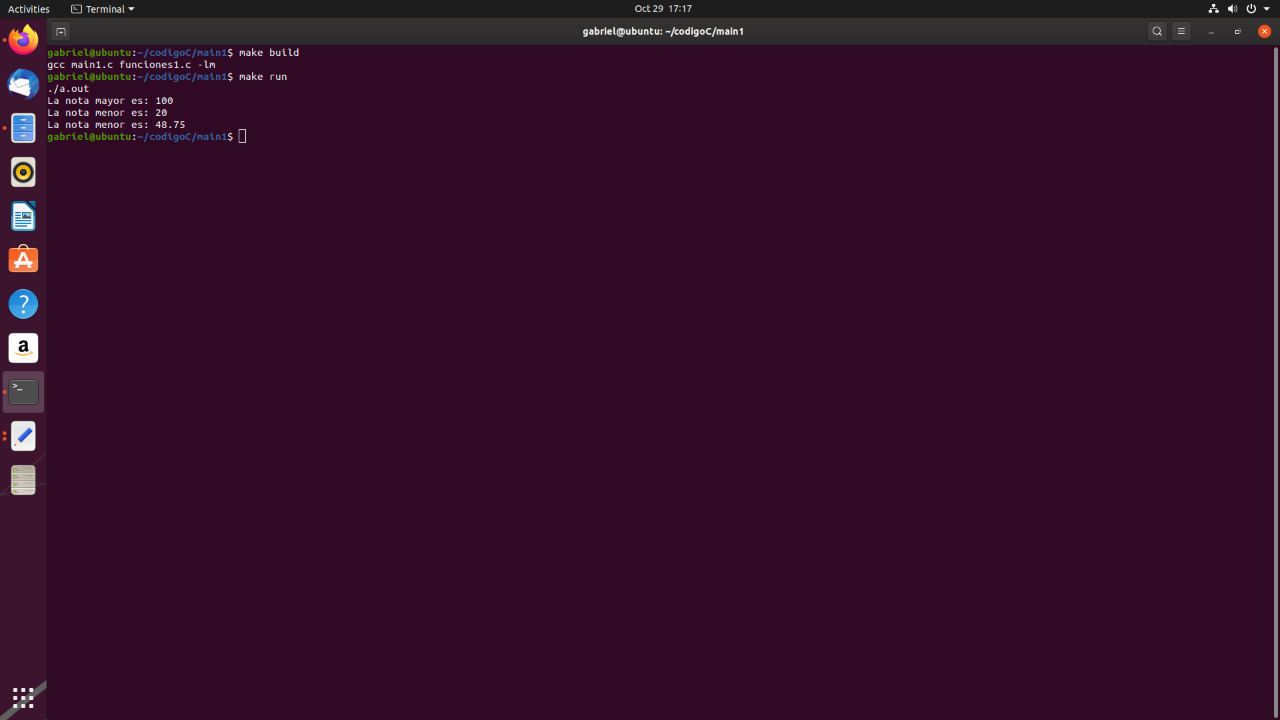
\includegraphics[trim= 30 550 800 30,clip,width=1.20\textwidth]{img/prueba3.jpg}
            \caption{Cuadro de compilación 3}
            \label{fig:my_label}
        \end{figure}
        
    \section{Conjetura de Collatz}
    En este problema se creó una función que permite verificar la conjetura de Collatz para cualquier número entero dado. Esto consiste en un proceso repetitivo, por lo cual se usó un ciclo while, en el que se da un número y a este se le hace cierta operación dependiendo si es par o impar. El resultado de cada operación se guarda hasta que el número llegue a ser 1 y finalmente se imprimen los resultados como una secuencia. En la figura 8 se observa la conjetura de Collatz para el número 6.
    
        \begin{figure}[H]
            \centering
            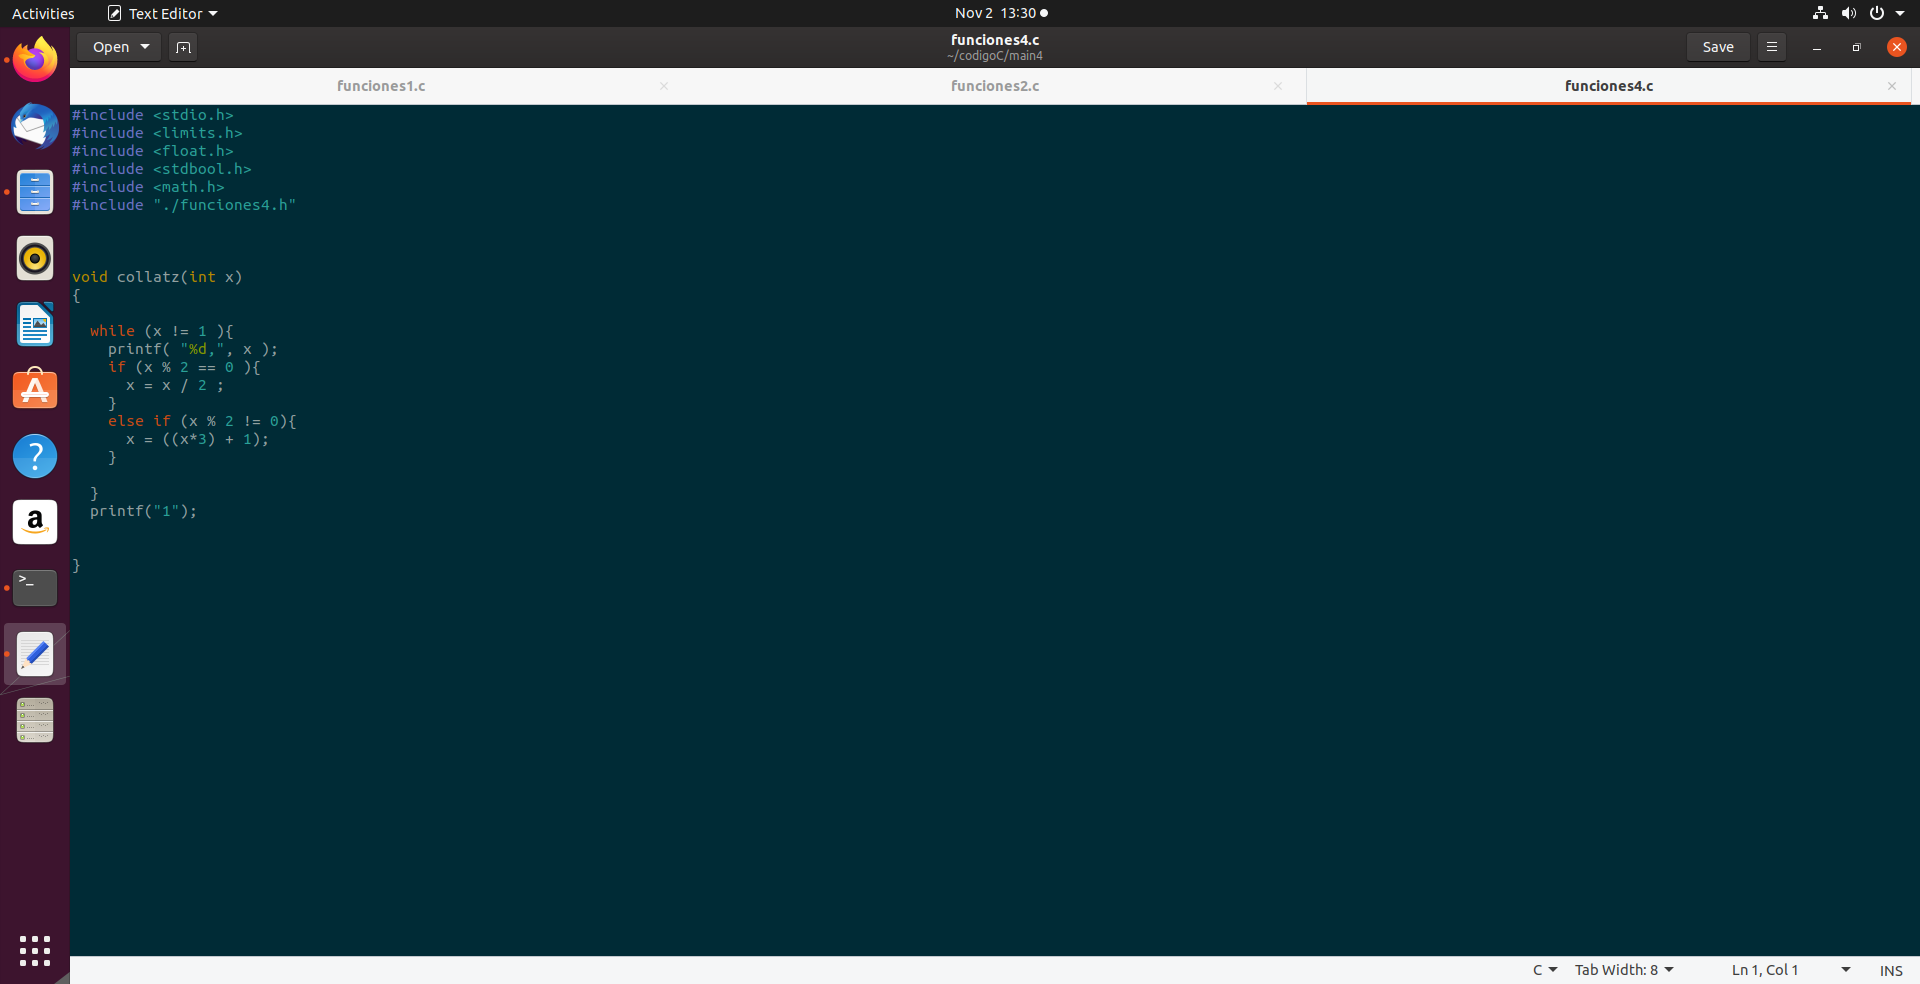
\includegraphics[trim= 50 400 1100 100,clip,width=1.20\textwidth]{img/punto4.png}
            \caption{Código para verificar la conjetura de Collatz}
            \label{fig:my_label}
        \end{figure}
        \begin{figure}[H]
            \centering
            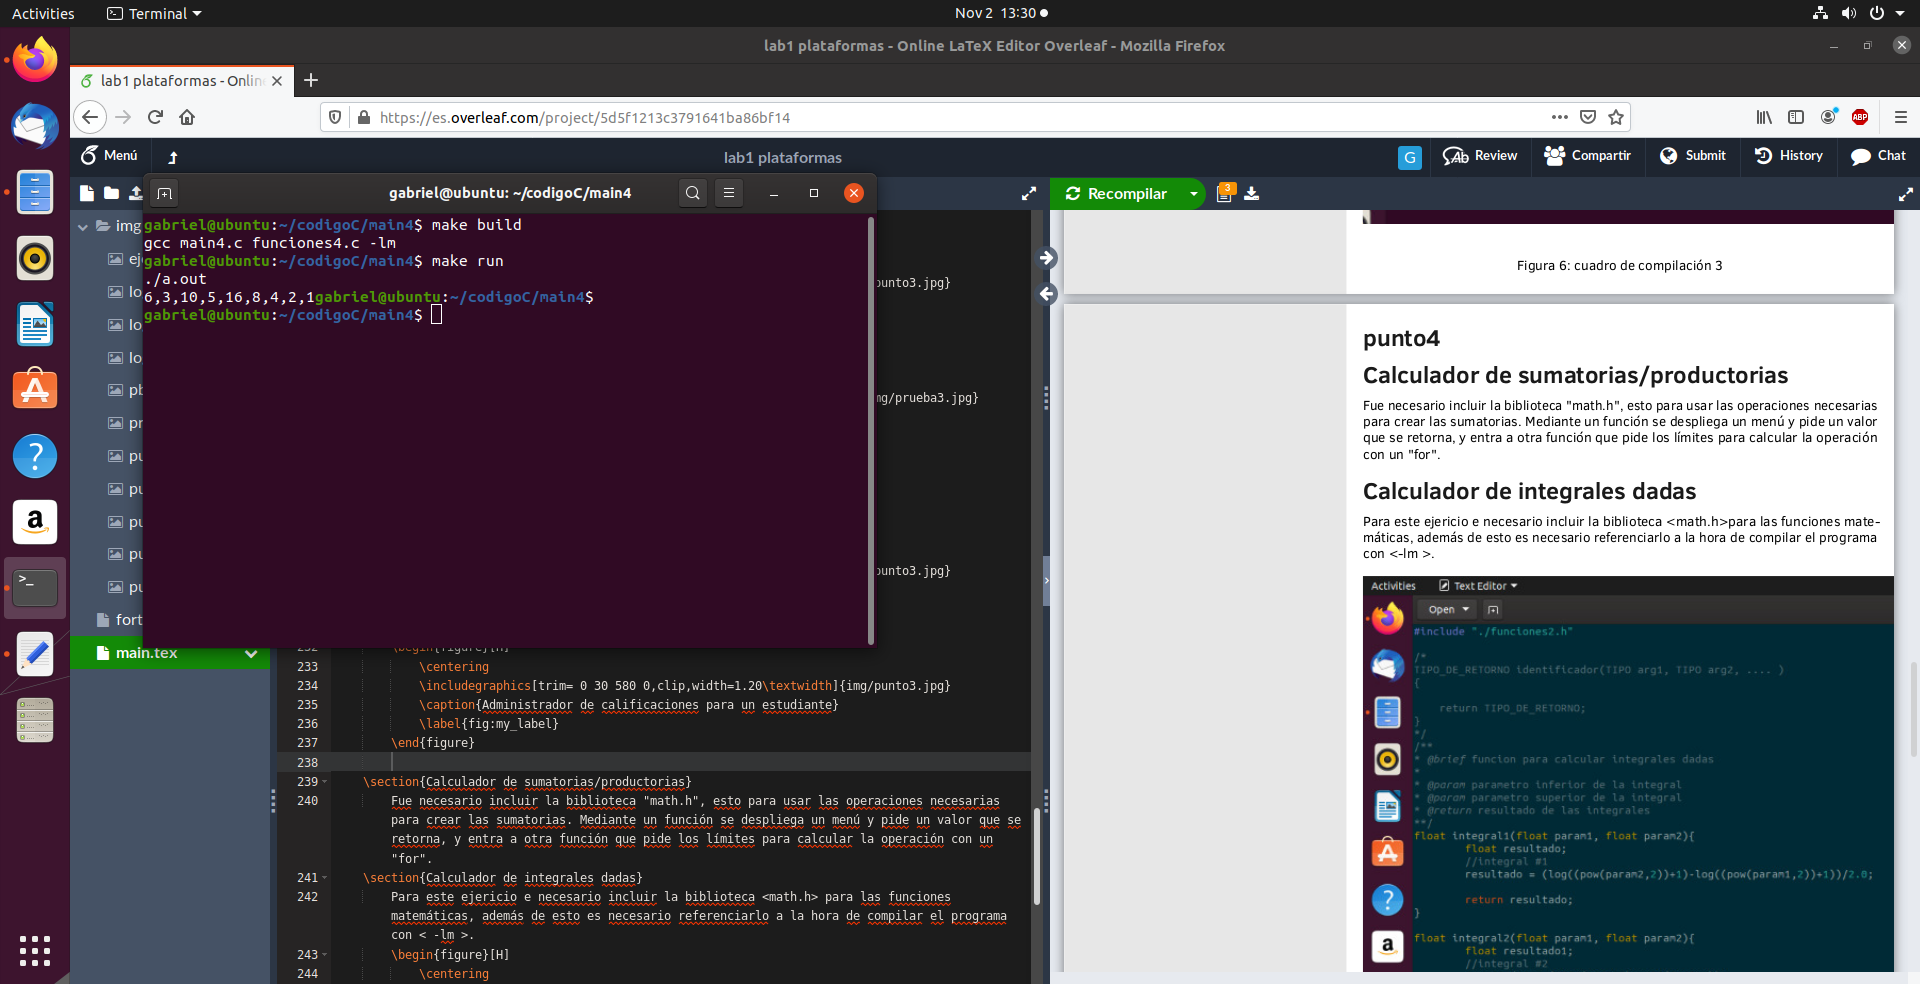
\includegraphics[trim= 130 550 980 100,clip,width=1.20\textwidth]{img/punto4-4.png}
            \caption{Conjetura de Collatz para el número 6}
            \label{fig:my_label}
        \end{figure}
        \newpage
    \section{Calculador de sumatorias/productorias}
        Fue necesario incluir la biblioteca "math.h", esto para usar las operaciones necesarias para crear las sumatorias. Mediante un función se despliega un menú y pide un valor que se retorna, y entra a otra función que pide los límites para calcular la operación con un "for".
        
        \begin{figure}[H]
            \centering
            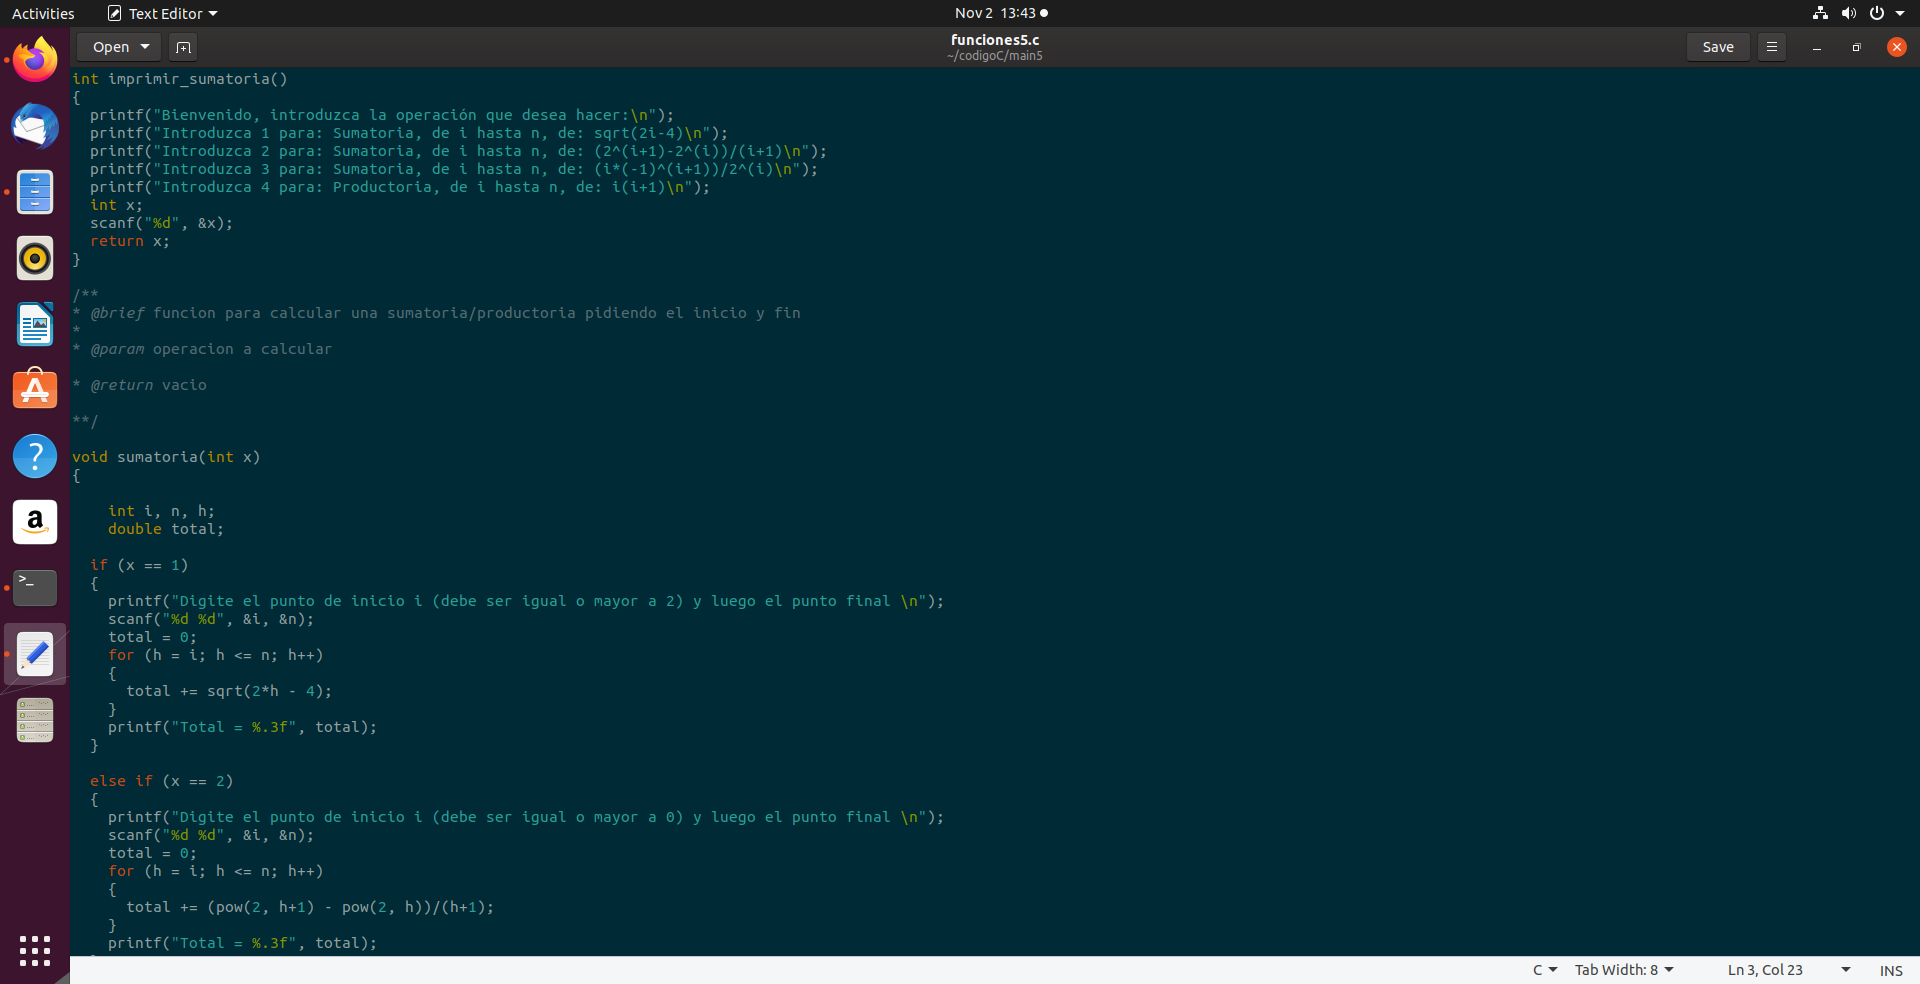
\includegraphics[trim= 50 0 580 50,clip,width=1.20\textwidth]{img/punto5.png}
            \caption{Calculadora de sumatorias/productorias}
            \label{fig:my_label}
        \end{figure}
        \begin{figure}[H]
            \centering
            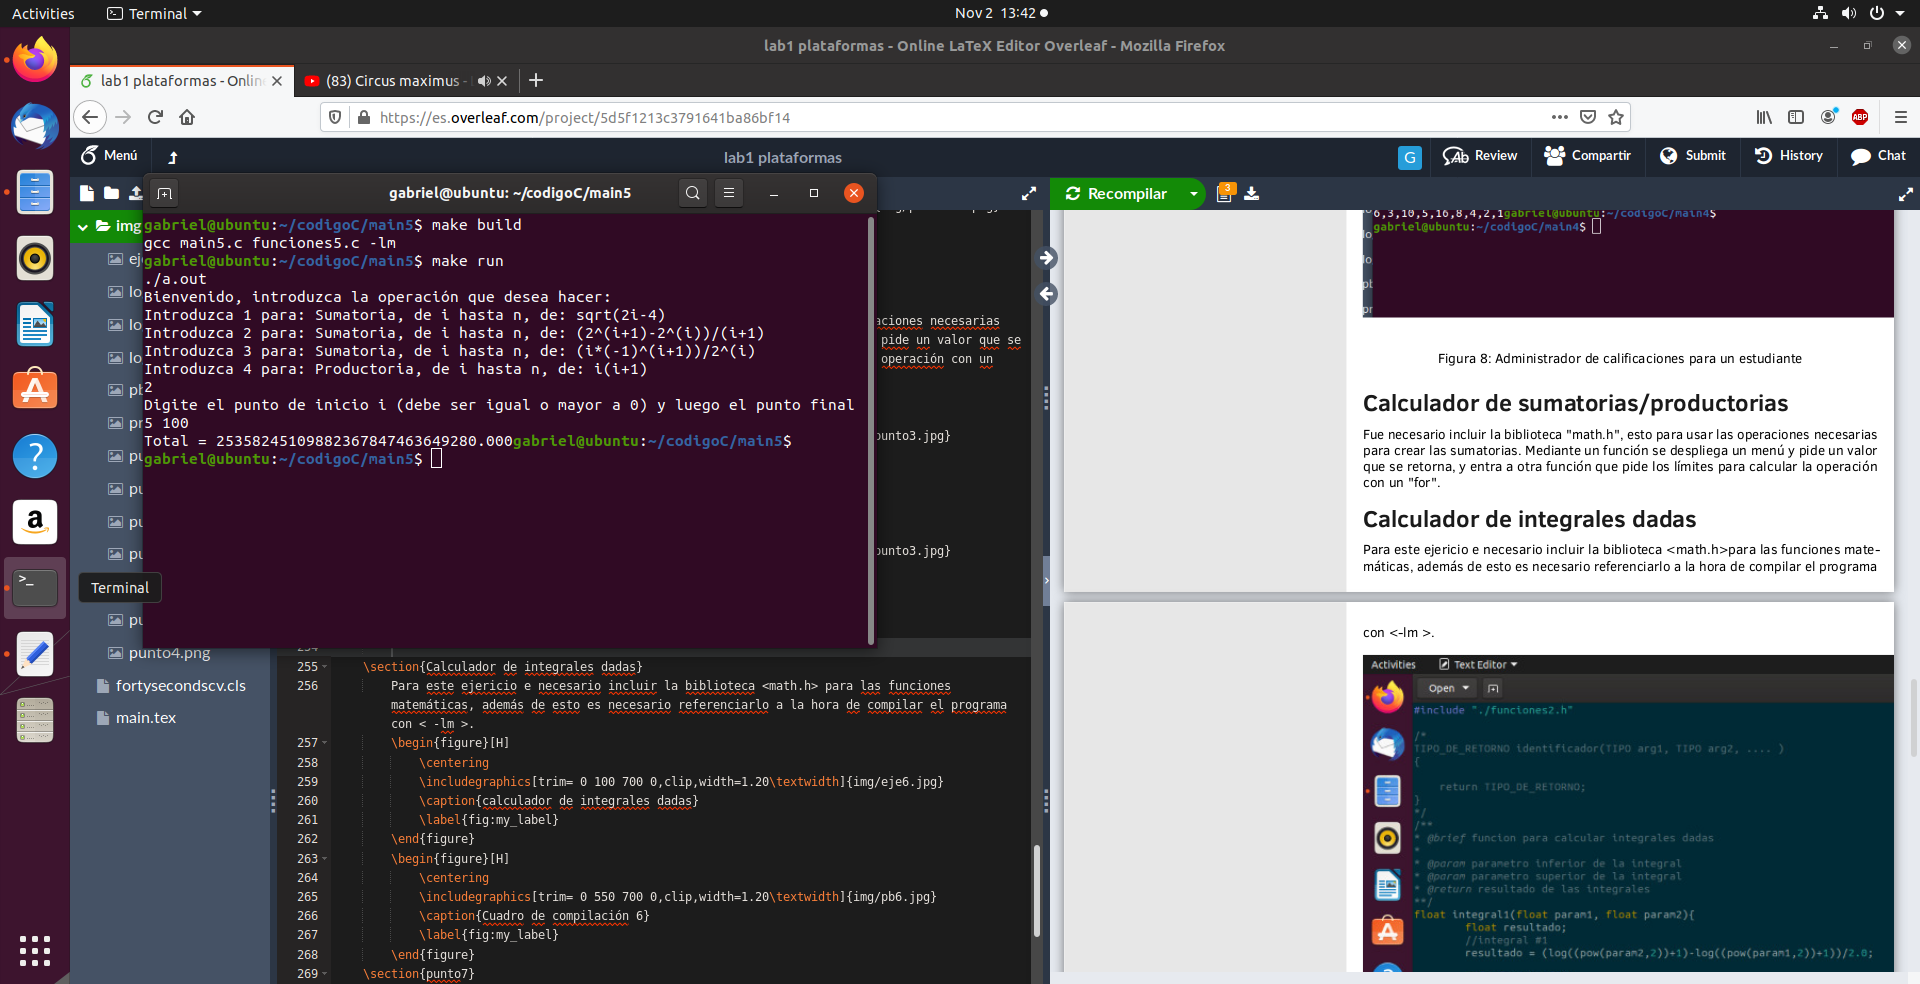
\includegraphics[trim= 130 500 915 180,clip,width=1.20\textwidth]{img/punto5-5.png}
            \caption{Cuadro de compilación para el ejercicio 5}
            \label{fig:my_label}
        \end{figure}
        \newpage
        
    \section{Calculador de integrales dadas}
        Para este ejericio e necesario incluir la biblioteca <math.h> para las funciones matemáticas, además de esto es necesario referenciarlo a la hora de compilar el programa con < -lm >.
        
        \begin{figure}[H]
            \centering
            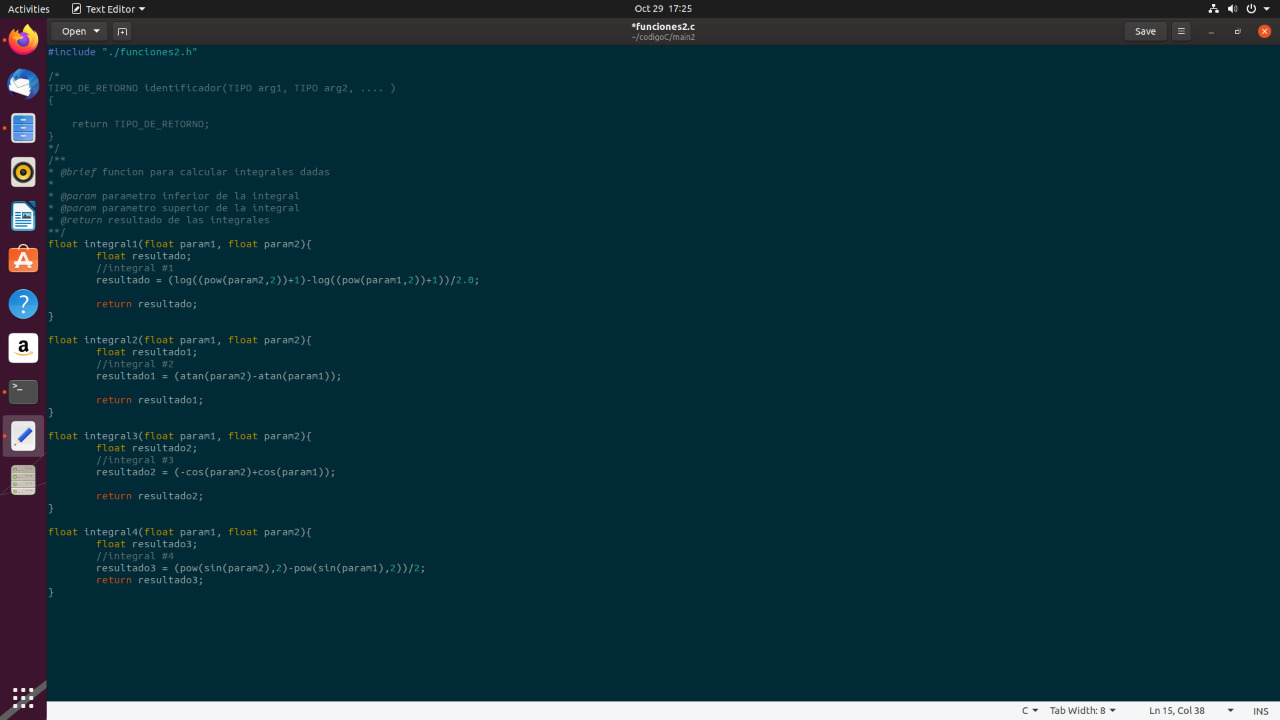
\includegraphics[trim= 30 120 600 30,clip,width=1.20\textwidth]{img/eje6.jpg}
            \caption{Calculador de integrales dadas}
            \label{fig:my_label}
        \end{figure}
        \begin{figure}[H]
            \centering
            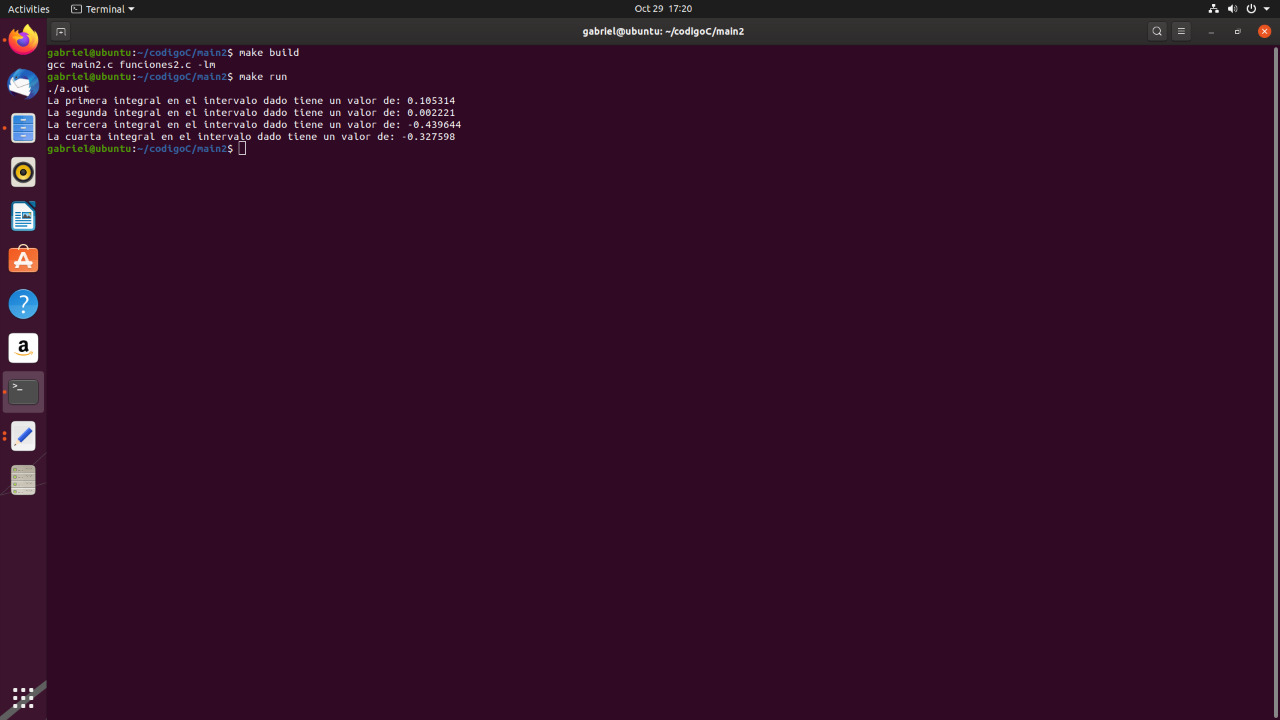
\includegraphics[trim= 0 550 700 0,clip,width=1.20\textwidth]{img/pb6.jpg}
            \caption{Cuadro de compilación para el ejercicio 6}
            \label{fig:my_label}
        \end{figure}
        \newpage
        
    \section{Permutaciones de los números de 1 hasta n}
        En este problema se creó un programa que imprime en pantalla las permutaciones de los números hasta el n dado. Para esto se utlizaron varios ciclos for en el que sus iteradores tienen que ser diferentes para que se logre asociar un iterador a cada dígito que está antes del número dado. En este caso se utilizó el número 3 de prueba.
    
        \begin{figure}[H]
            \centering
            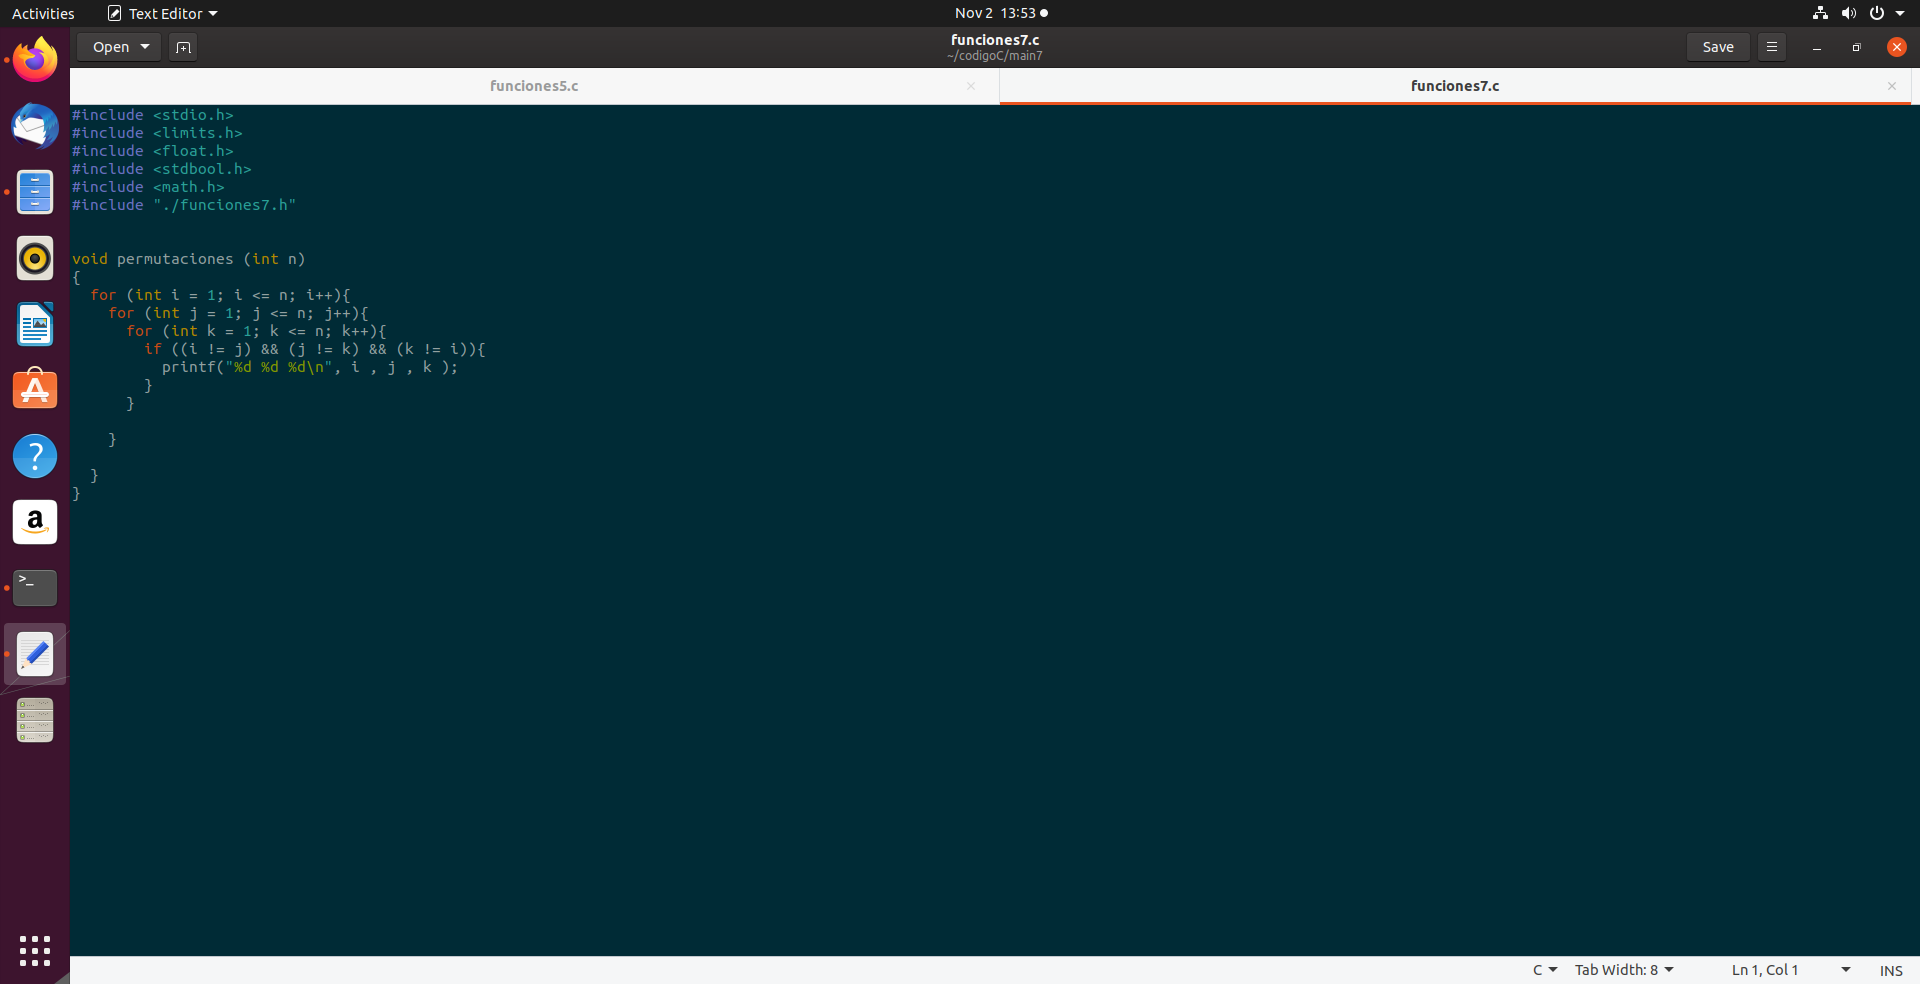
\includegraphics[trim= 50 480 980 50,clip,width=1.20\textwidth]{img/punto7.png}
            \caption{Código para obtener permutaciones de un número}
            \label{fig:my_label}
        \end{figure}\begin{figure}[H]
            \centering
            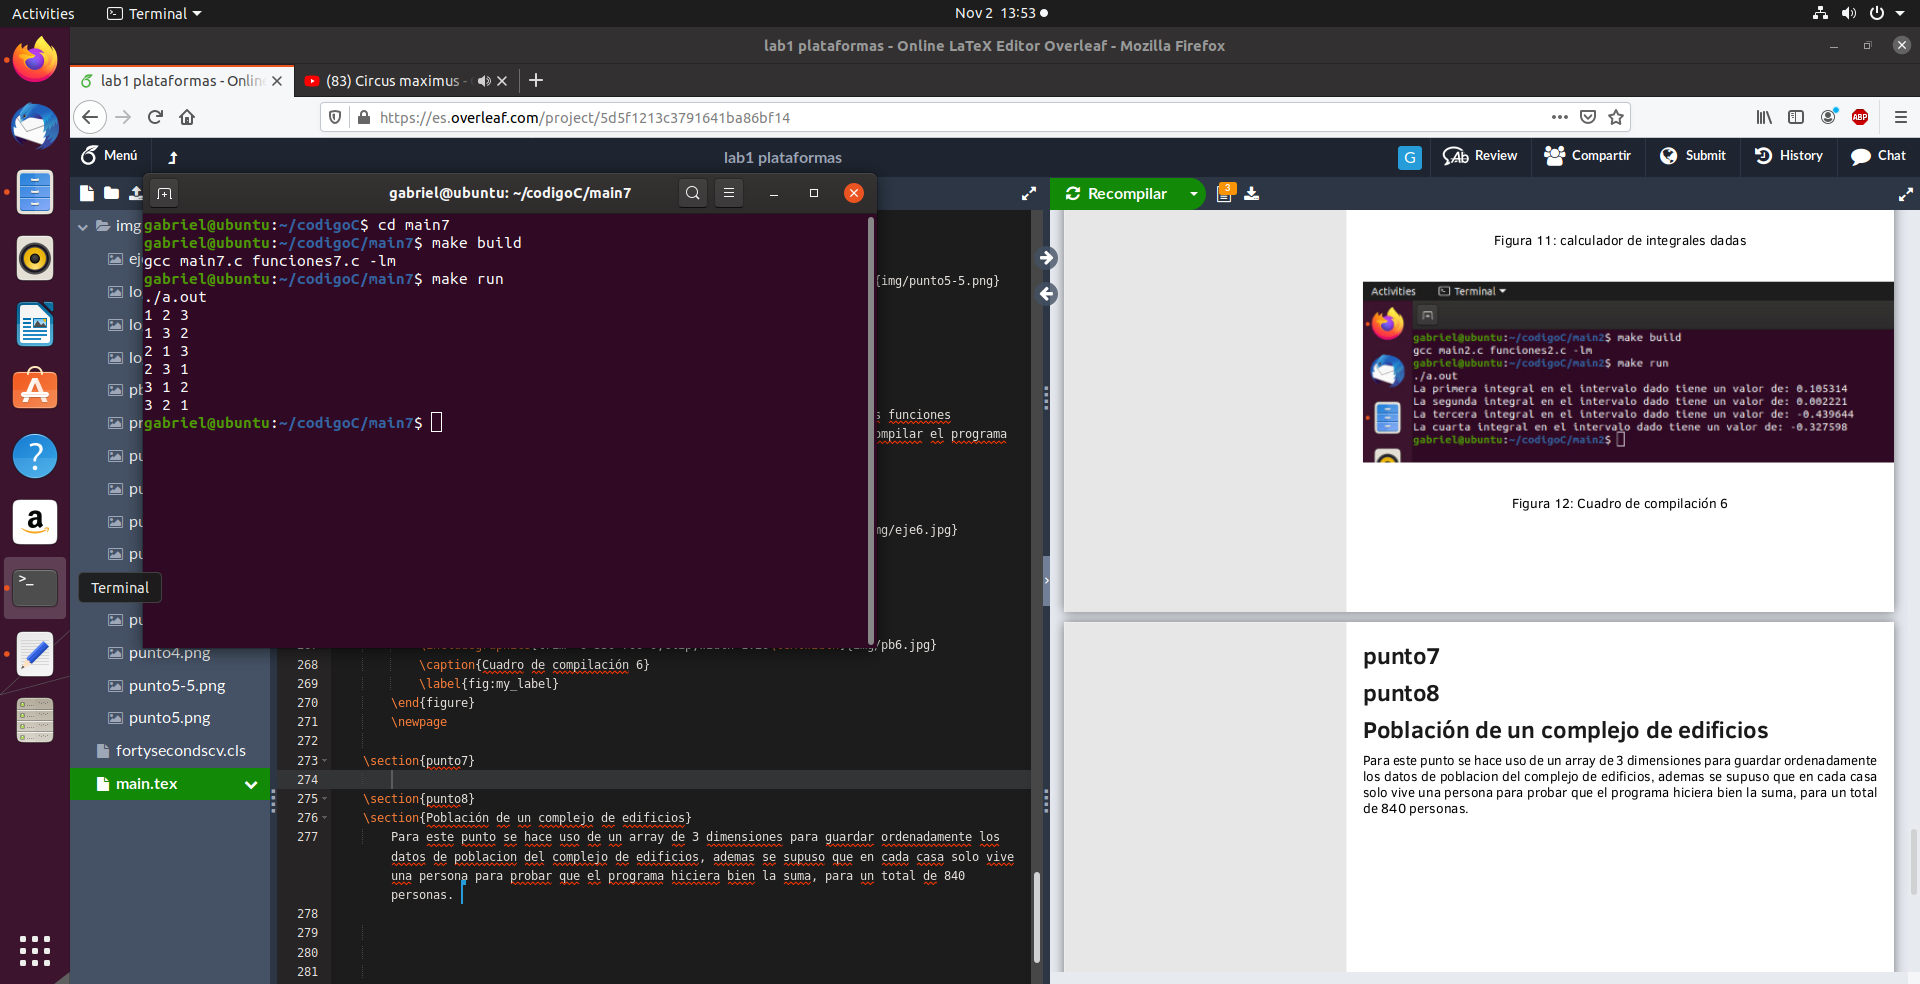
\includegraphics[trim= 135 500 980 150,clip,width=1.20\textwidth]{img/punto7-7.png}
            \caption{Permutaciones de los números de 1 hasta 3}
            \label{fig:my_label}
        \end{figure}
        \newpage
        
    \section{Subconjuntos propios no vacios de 1 hasta n}
        Para este ejercicio, mediante un proceso iterativo, se logran imprimir los subconjuntos de 1 hasta n, donde n es un parámetro de la función. Para lograr esto fue necesario la utilización de condicionales y ciclos.
    
        \begin{figure}[H]
            \centering
            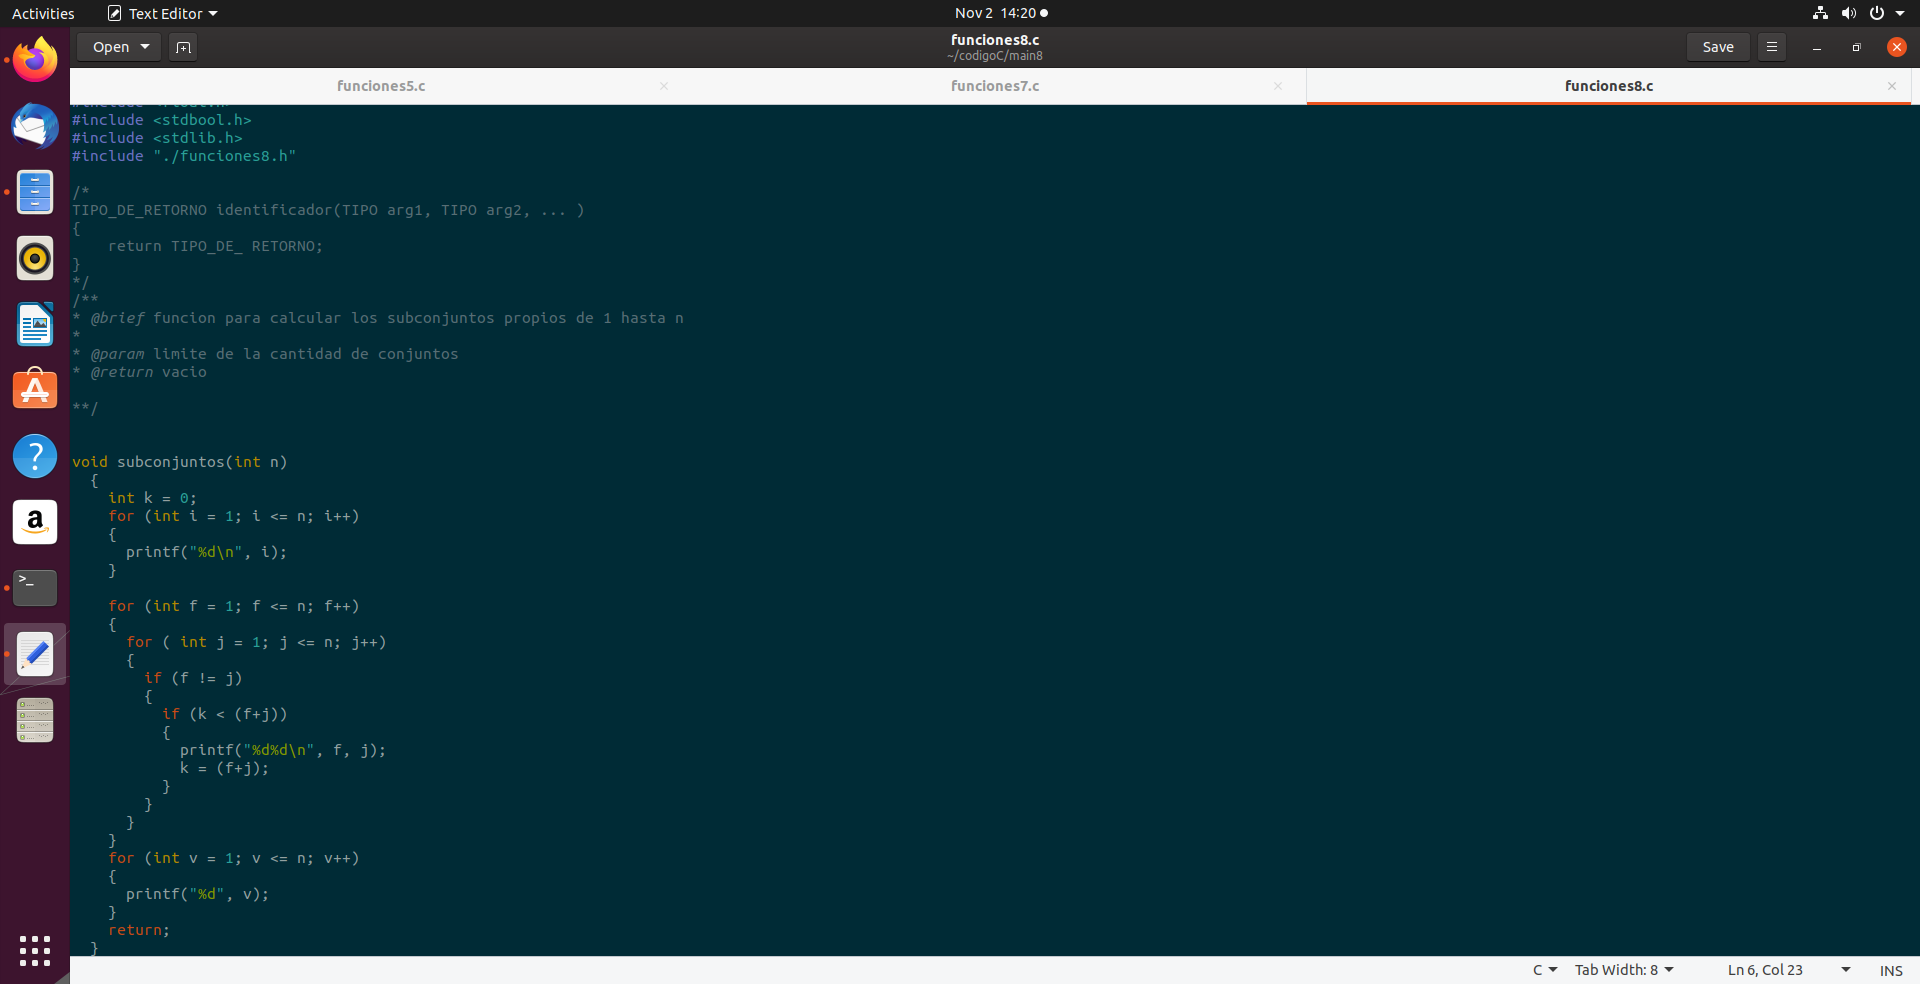
\includegraphics[trim= 50 10 800 90,clip,width=1.20\textwidth]{img/punto8.png}
            \caption{Código de la impresora de subconjuntos propios}
            \label{fig:my_label}
        \end{figure}
        \begin{figure}[H]
            \centering
            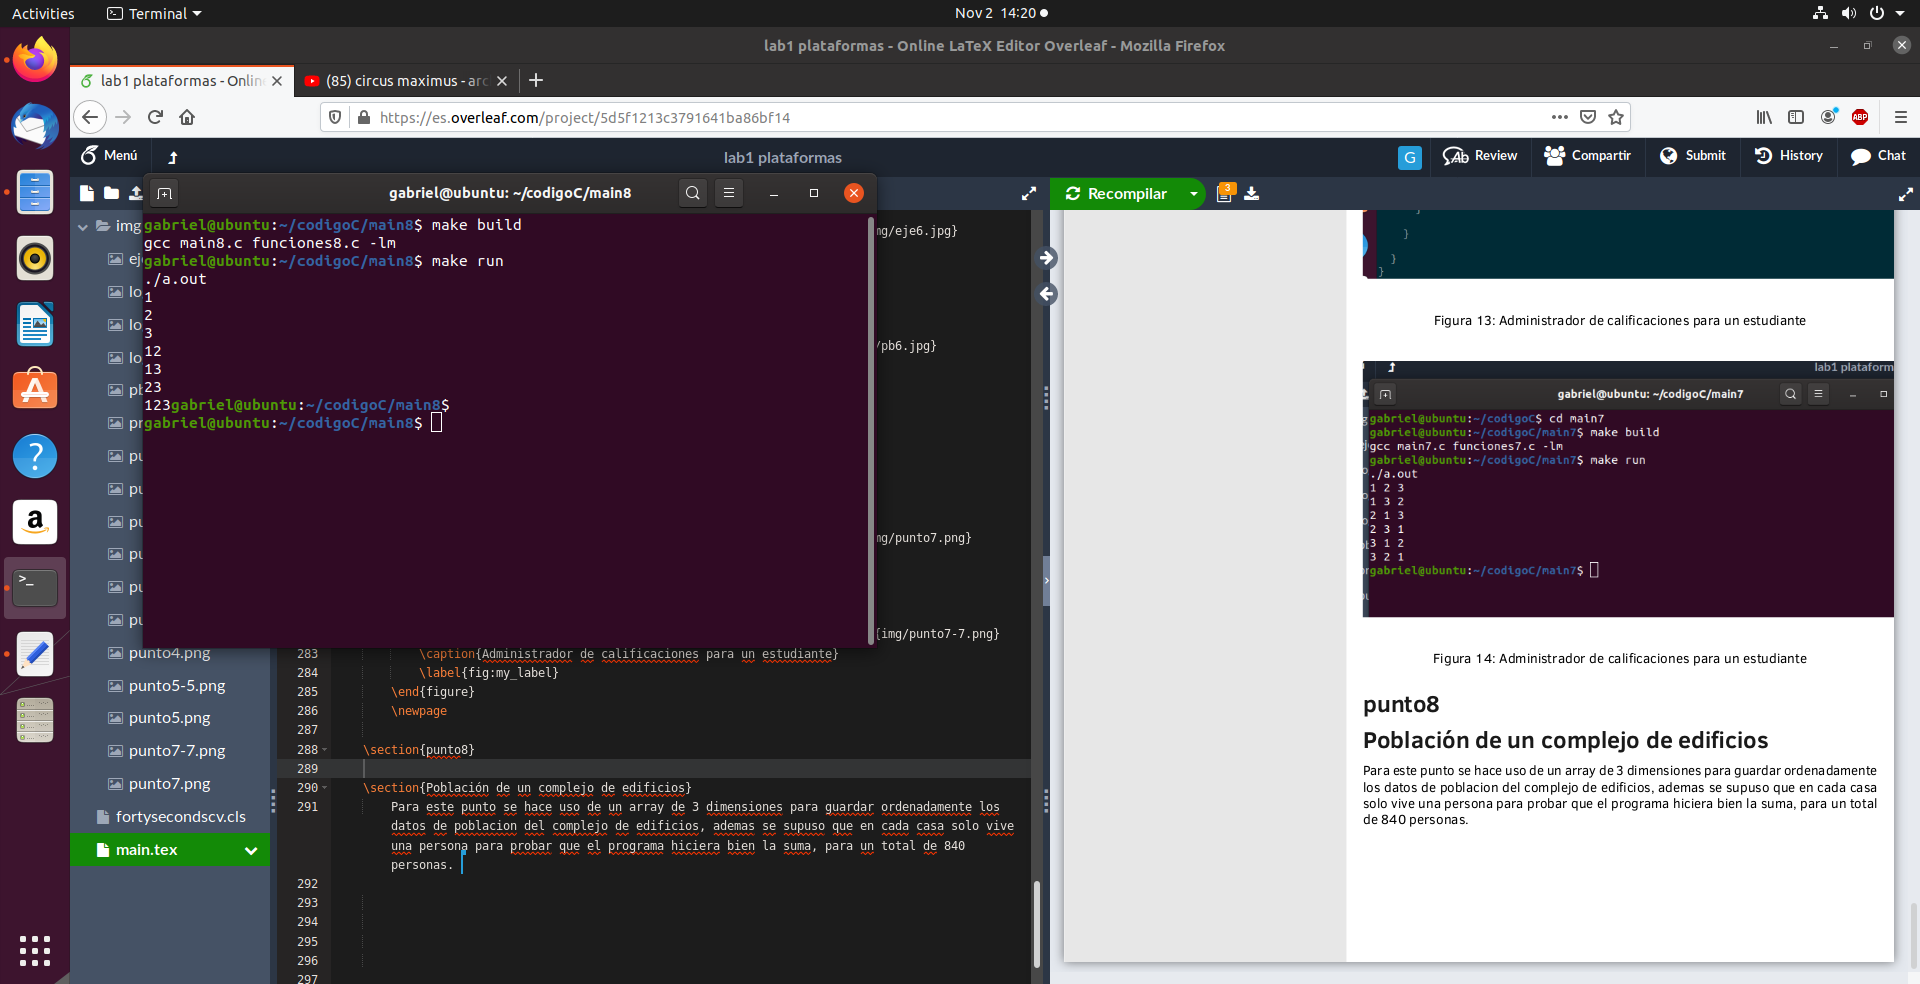
\includegraphics[trim= 125 500 980 150,clip,width=1.20\textwidth]{img/punto8-8.png}
            \caption{Cuadro de compilación para el ejercicio 8}
            \label{fig:my_label}
        \end{figure}
    \newpage
    \section{Población de un complejo de edificios}
        Para este punto se hace uso de un array de 3 dimensiones para guardar ordenadamente los datos de poblacion del complejo de edificios, ademas se supuso que en cada casa solo vive una persona para probar que el programa hiciera bien la suma, para un total de 840 personas. 
        
        \begin{figure}[H]
            \centering
            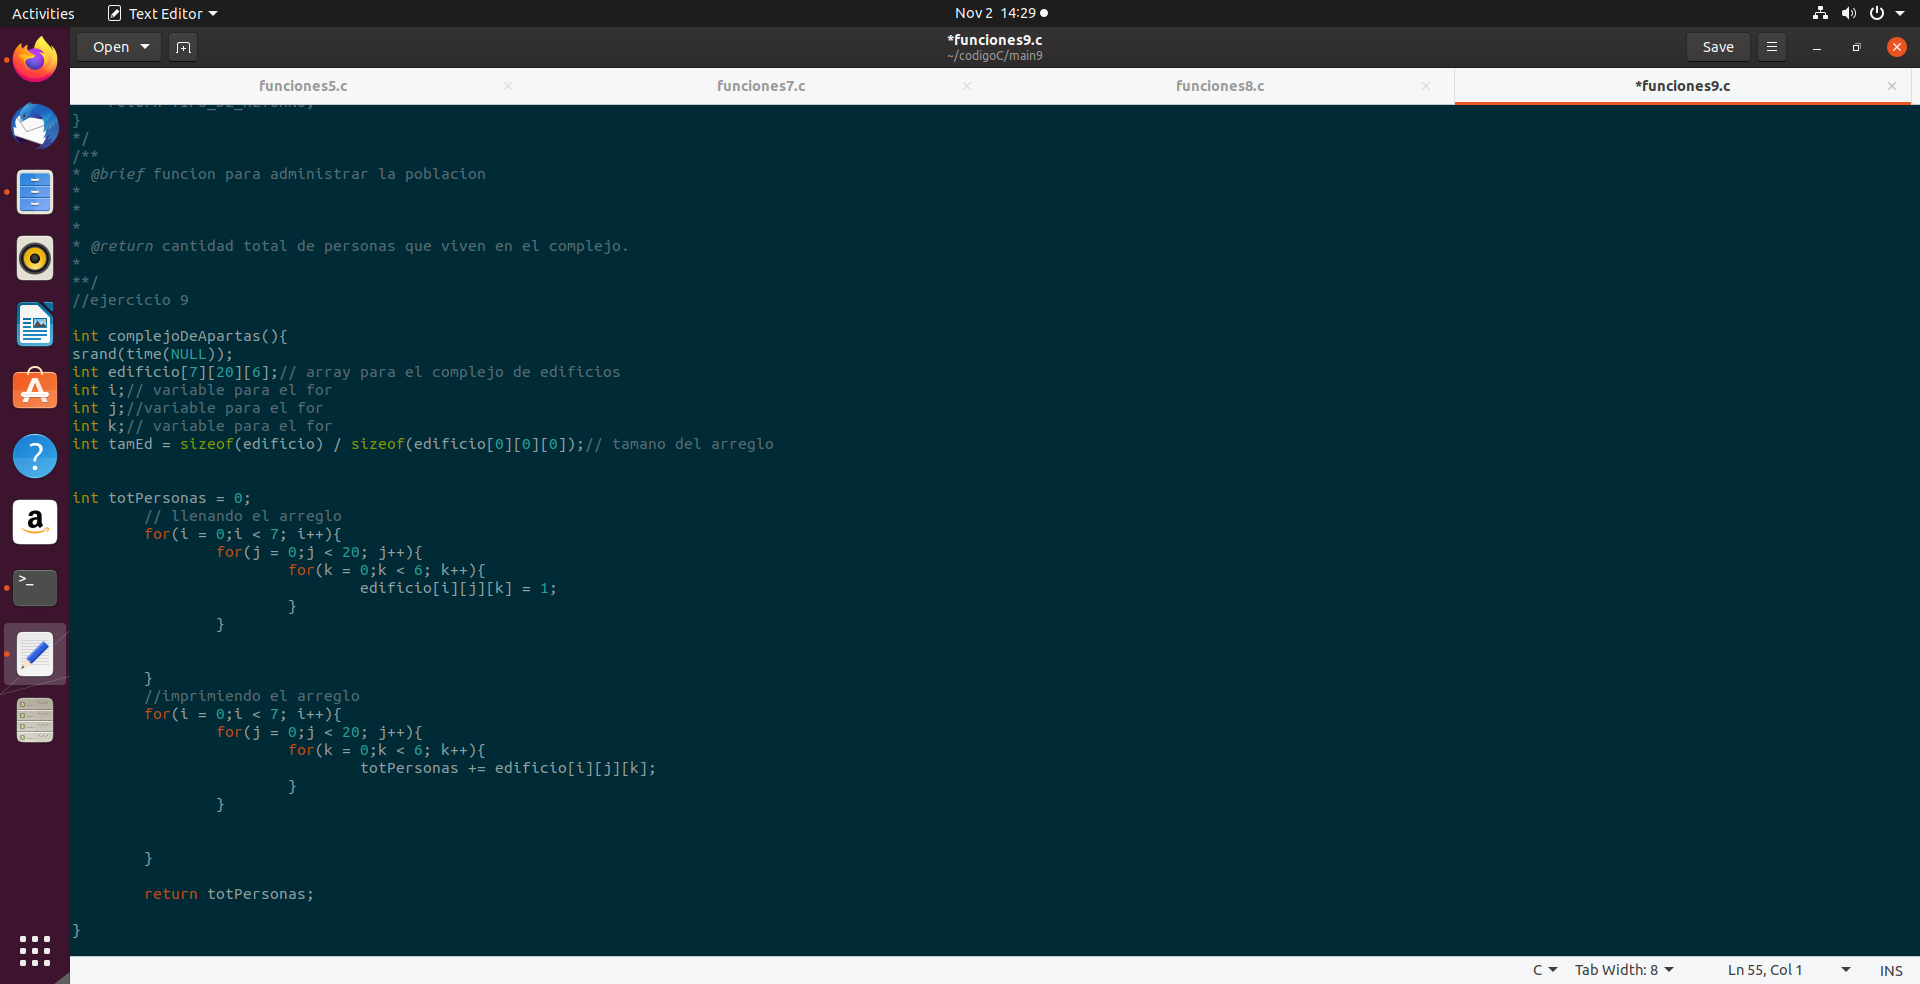
\includegraphics[trim= 50 30 780 90,clip,width=1.20\textwidth]{img/punto9.png}
            \caption{Administrador para la cantidad de poblacion de un edifcio}
            \label{fig:my_label}
        \end{figure}
        \begin{figure}[H]
            \centering
            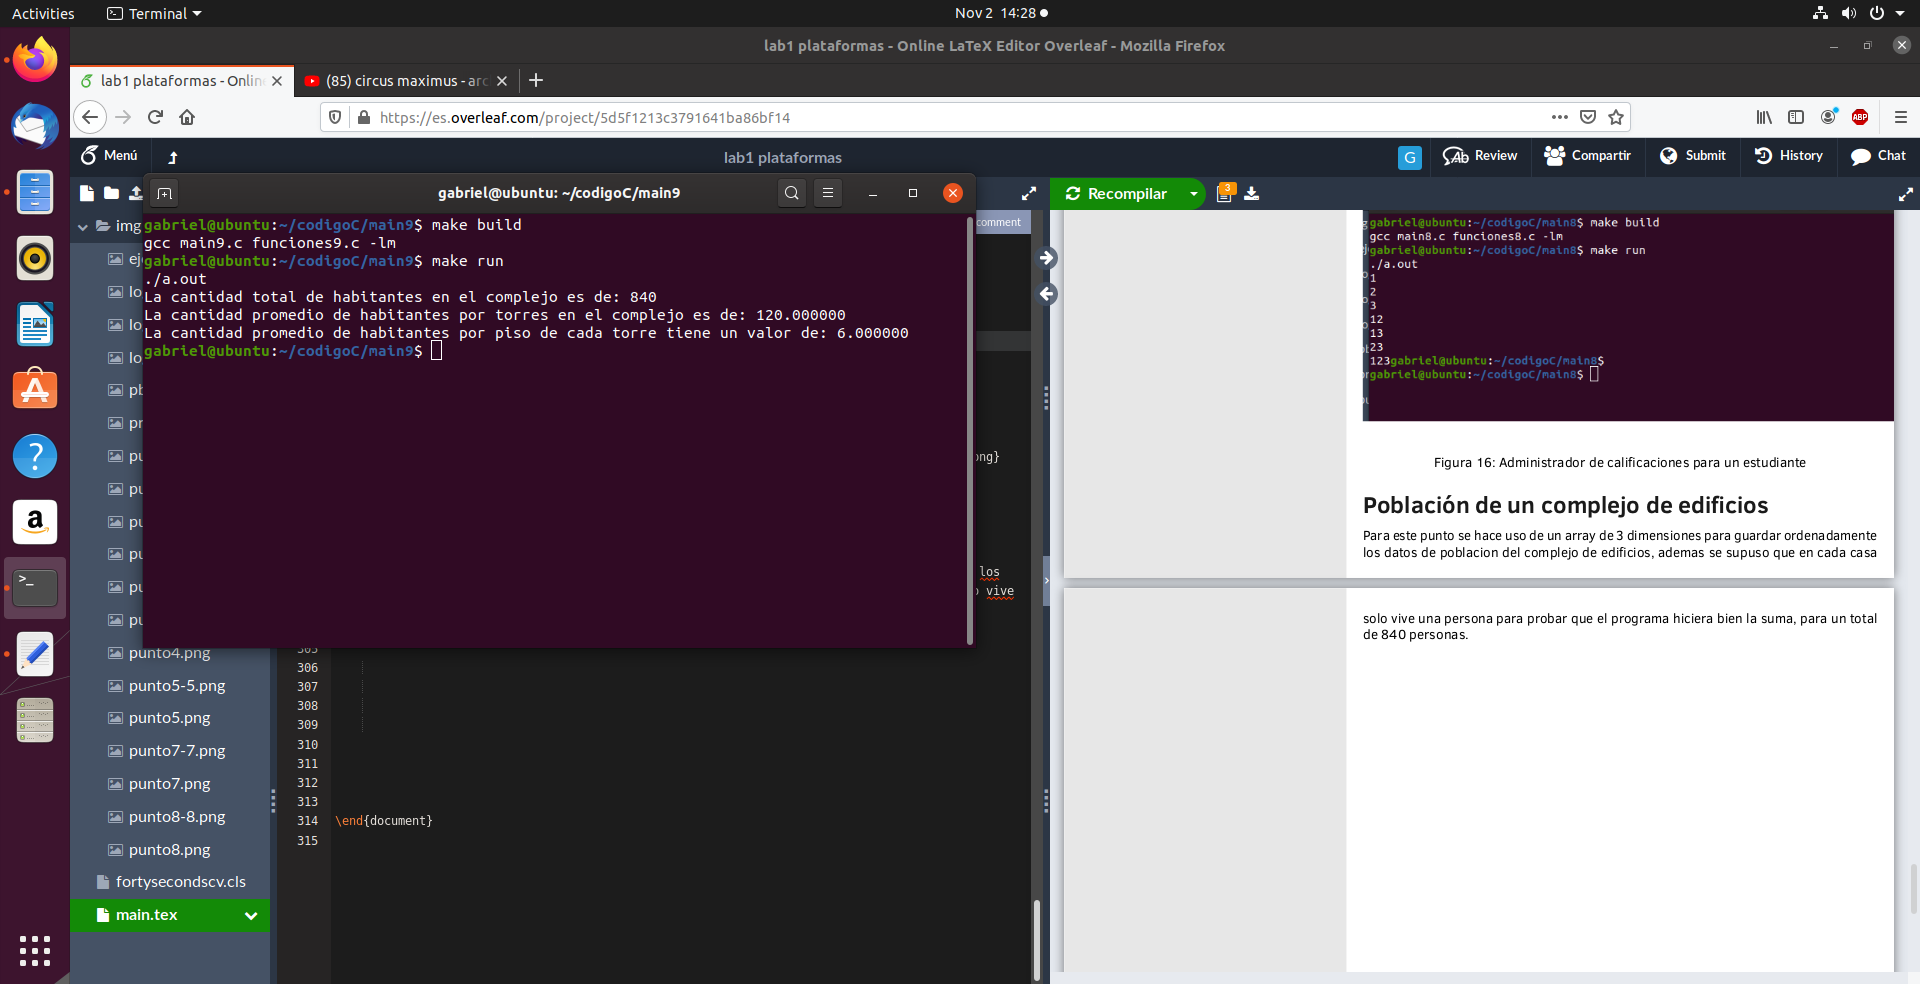
\includegraphics[trim= 135 500 850 150,clip,width=1.20\textwidth]{img/punto9-9.png}
            \caption{Salida del programa}
            \label{fig:my_label}
        \end{figure}

        
        
        
        
    
    

    
\end{document}
